\subsection {Session 10, Exercise 5}

\lineparagraph {Exercise}

We are moving on the squares of an $n \times n$ chessboard from the lower left corner to the upper right corner so that in one step we can move to the neighboring square to the right or up. However, there are some squares given that are ''forbidden'', that is we cannot step on them. Give a dynamic programming procedure that determines how many different ways can we get to the upper right corner.

\lineparagraph {Solution}

\textbf{What is Dynamic Programming?}

\begin{itemize}
    \item Dynamic programming is just smart recursion. I like to give the example of calculating Fibonacci-numbers to explain what this means.
    \item Fibonacci-numbers are defined recursively. The first and second Fibonacci-numbers are $1$ and $1$. If we denote the $i$th Fibonacci-number with $F[i]$, then $F[1]=1, F[2]=1$. After that, each Fibonacci-number is the sum of the previous two: $F[i] = F[i-1] + F[i-2]$, for $i\geq{}2$.
    \item If we wrote a program to calculate these numbers, we could write a recursive function like so:
\end{itemize}


\begin{minted}[linenos]{c++}
int f(int index) {
  if(index == 1 || index == 2) {
    return 1;
  }
  return f(index-1) + f(index-2);
}
\end{minted}

\begin{itemize}
    \item Let's take a look at the function calls for $f(n)$:
\end{itemize}

\begin{center}
    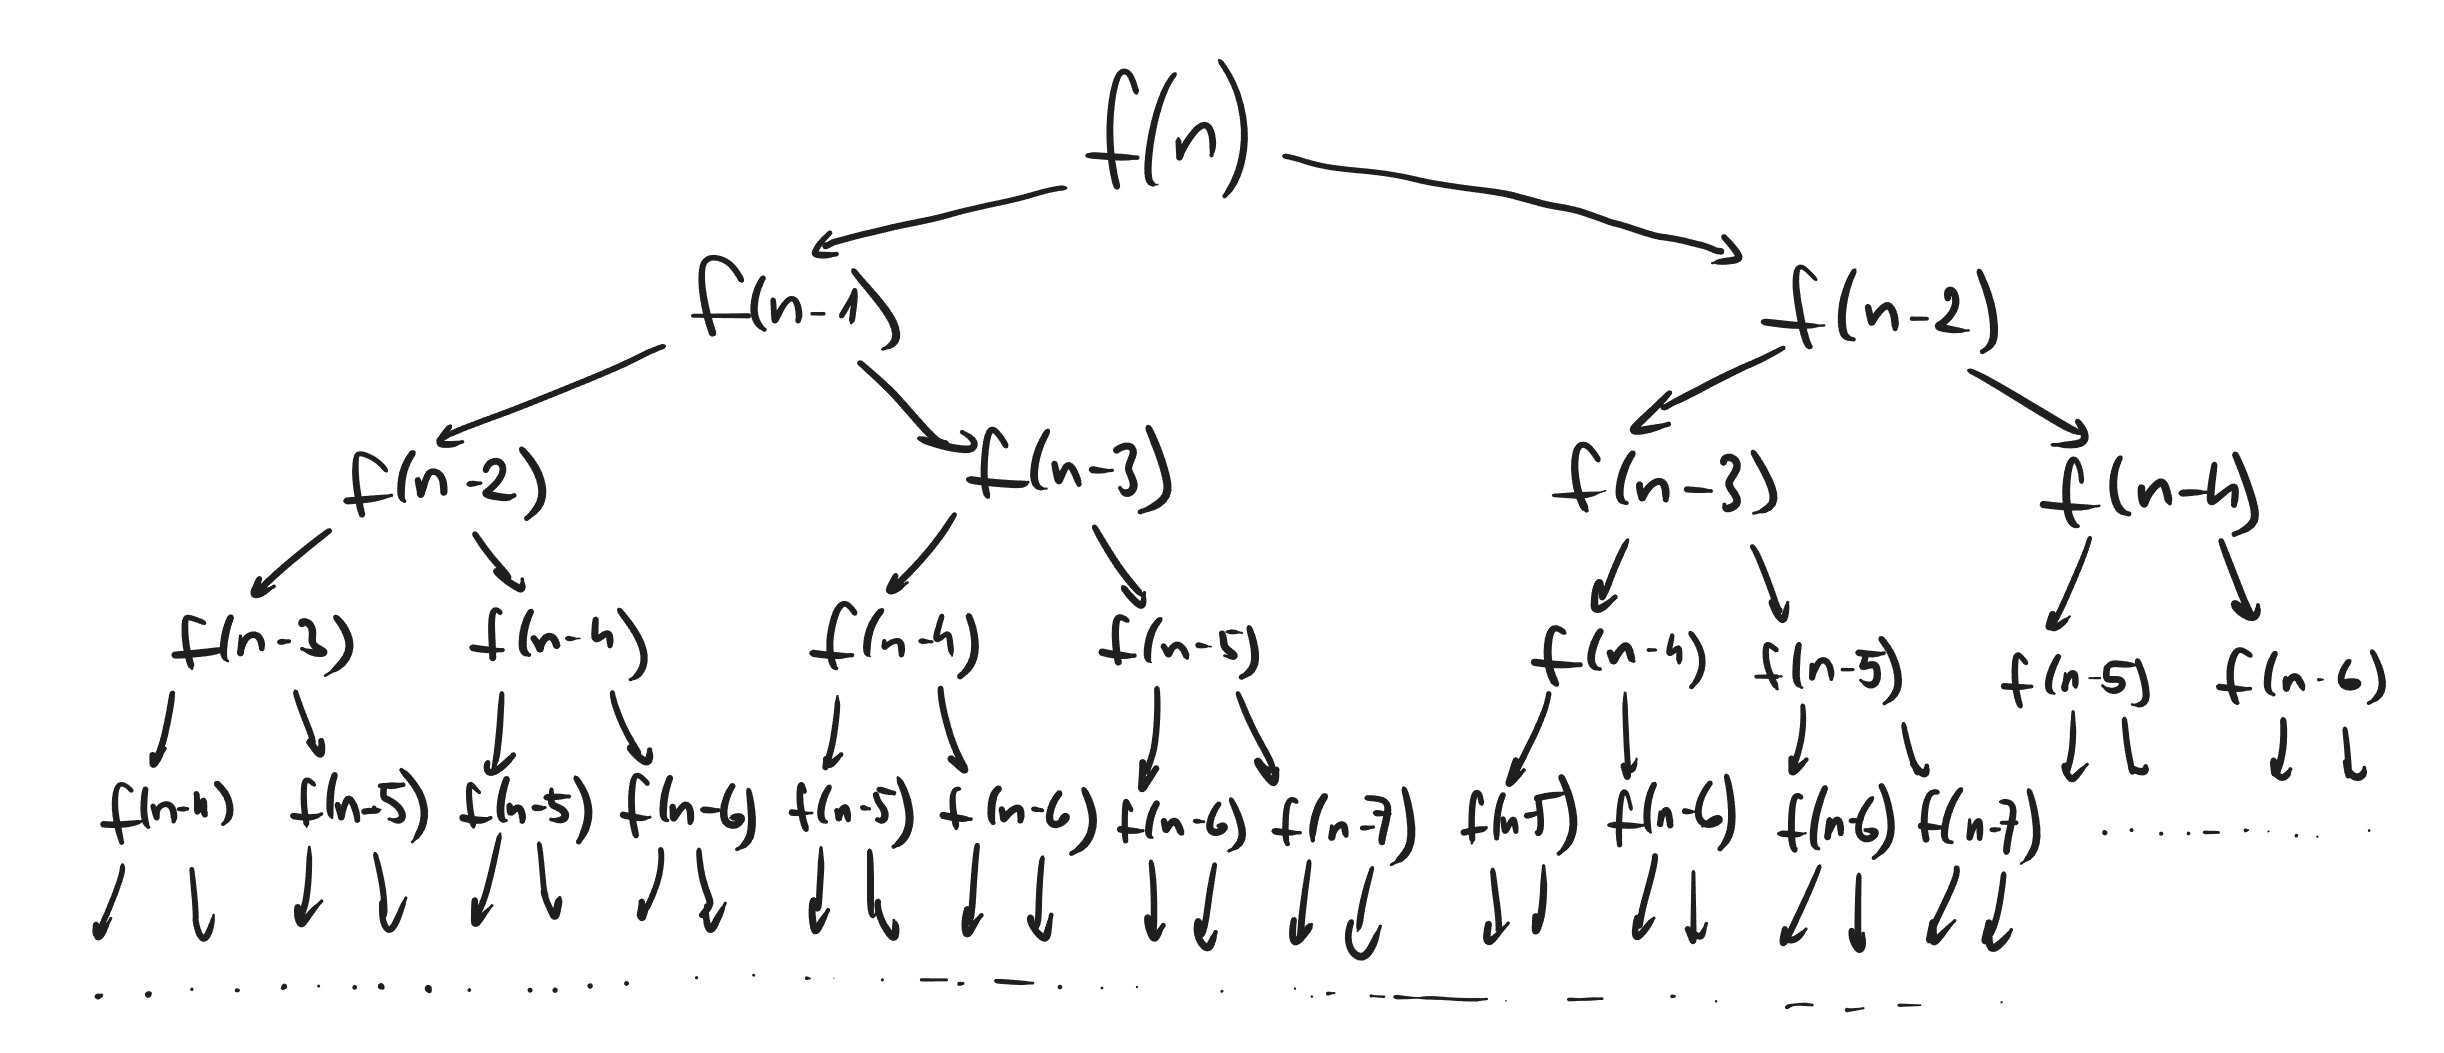
\includegraphics[width=\linewidth]{10/05/fibonacci_recursive.png}
\end{center}

\begin{itemize}
    \item We calculate the $(n-2)$th Fibonacci number two times, the $(n-3)$th 3 times, the $(n-4)$th 5 times, the $(n-5)$th 7 times (1 of which is not plotted), and so on... Quite wasteful isn't it?
    \item Bonus points if you noticed, that the number of times we recalculate the $(n-i)$th Fibonacci number is actually the $i$th Fibonacci number. Double bonus points if you can prove this. :)
    \item Wouldn't it be better if we just remembered our calculations and whenever we needed them again, we could just pull the information out of memory? Let's create an array, where we store the Fibonacci numbers we have already calculated!
\end{itemize}

\begin{minted}[linenos]{c++}
#include<vector>

int N = 100;
// Initializes vector of size N of 0's.
// (N+1 so indexing is 1-based for convenience.)
vector<int> T = new vector<int>(N+1);

// Base cases.
T[1] = 1;
T[2] = 1; 

int f(int index) {
  if (T[index]) { // If T[index] is already calculated, we return it.
    return T[index];
  }
  else { // Otherwise T[index] = 0, so not yet calculated: calculate it, store it, then return it.
    T[index] = f(index-1) + f(index-2);
    return T[index];
  }
}
\end{minted}

\begin{itemize}
\item To simplify this a bit:
\end{itemize}

\begin{minted}[linenos]{c++}
#include<vector>

int N = 100;
vector<int> T = new vector<int>(N+1);

T[1] = 1;
T[2] = 1; 

int f(int index) {
  if (!T[index]) {
    T[index] = f(index-1) + f(index-2);
  }
  return T[i];
}
\end{minted}

\begin{itemize}
    \item If we look back on the branching of the calculation of $f(n)$, we just cut off all right-side branches:
\end{itemize}

\begin{center}
    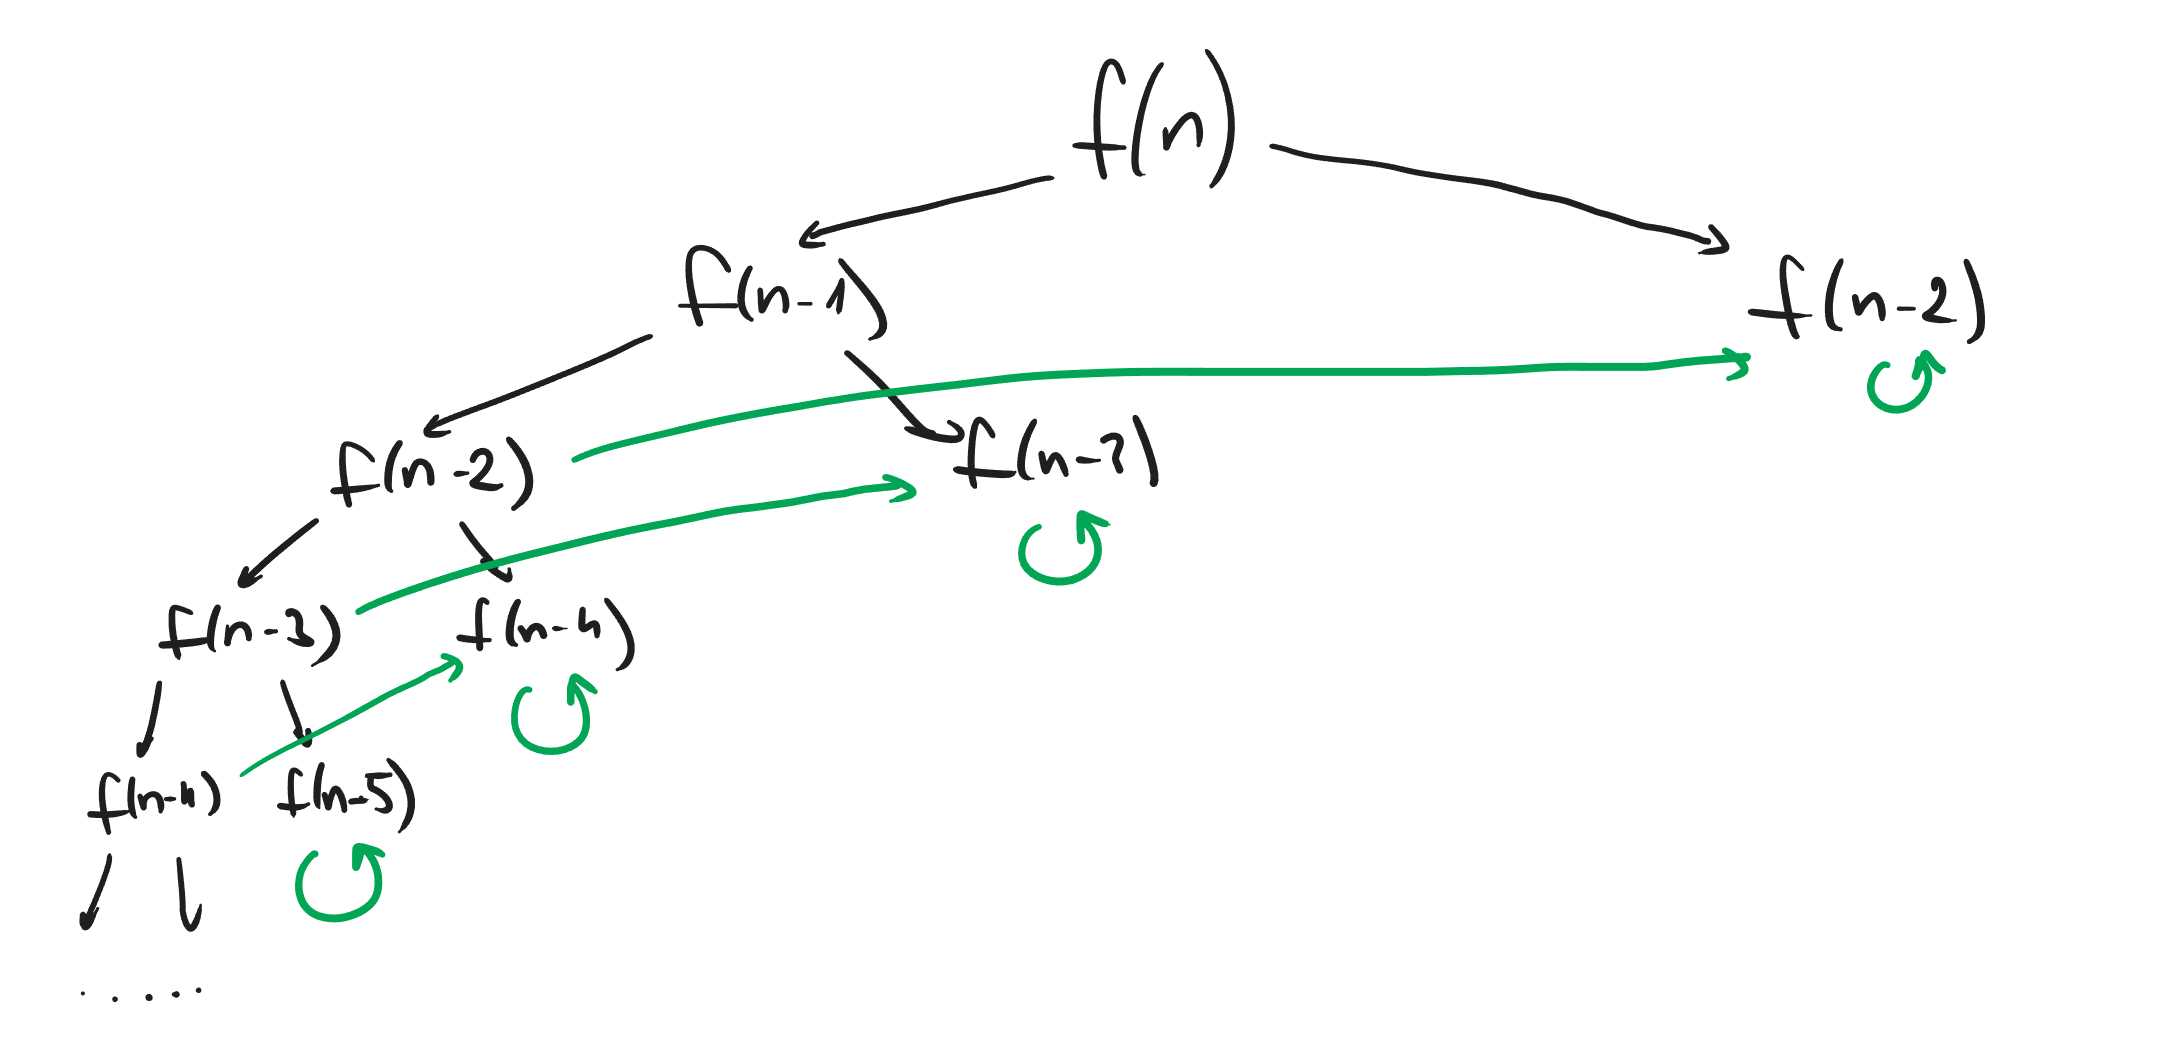
\includegraphics[width=\linewidth]{10/05/fibonacci_cutoff.png}
\end{center}

\begin{itemize}
    \item So essetially, our recursion turned into a single-branching, insted of a double-branching:
\end{itemize}

\begin{center}
    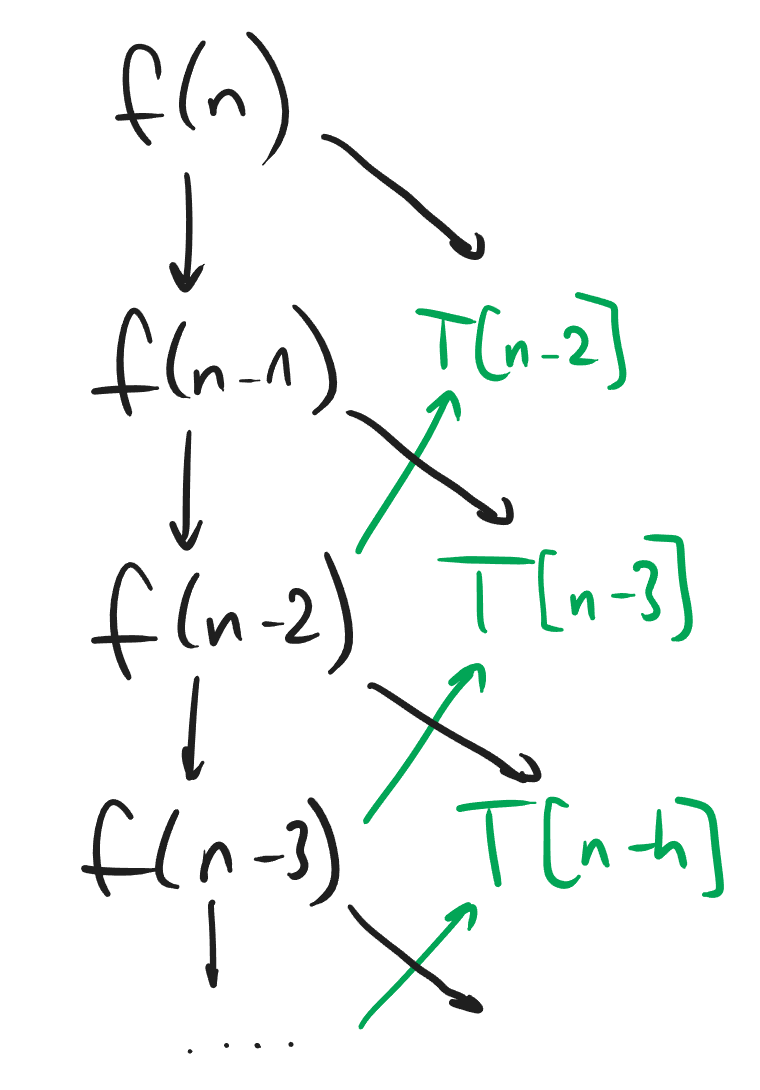
\includegraphics[width=0.5\linewidth]{10/05/fibonacci_single.png}
\end{center}

\begin{itemize}
    \item What we have done here is called \textbf{memoization} (and the missing \textbf{r} is not a typo).
    \item For example in Python, we can add memoization to any function without writing additional code, by using a decorator, called \href{https://docs.python.org/3/library/functools.html#functools.cache}{@cache}.
    \item While memoization allowed us to cut the $O(2^n)$ runtime into $O(n)$, so this runs fast, there is still one problem that remains: we are still abusing and wasting the stack.
    \item Every time a function is called, a block of memory is reserved on the stack, for things like storing the internal variables, the return value and the instruction pointer to return to. The stack size is around $1-2$ MB at most. Some programming languages, like Python limit recursion depth to around 1000, while other languages like C++ let you exhaust it at your own will, resulting in a stack overflow.
    \item This means that using this approach, we won't be able to calculate Fibonacci-numbers with an index greater than 1000.
    \item However, instead of calculating top-down, starting from the $n$th number, back to $1$ using recursion, we could instead calculate bottom-up, by filling out the $T$ array starting from the index $1$ all the way to $n$, like this:
\end{itemize}


\begin{minted}[linenos]{c++}
#include<vector>

int N = 100;
vector<int> T = new vector<int>(N+1);

T[1] = 1;
T[2] = 1;

for(int index = 3; index <= n; ++index) {
    T[index] = T[index-1] + T[index-2]; // The previous indexes have already been calculated.
}

// Result is in T[100].
\end{minted}

\begin{itemize}
\item We no longer need a recursive function, since we intentionally fill out the T array in an order, where the values needed to calculate the current value are already available.
\item So Dynamic Programming = Recursion + Memoization (runtime optimization) + a Bottom-up approach (memory usage optimization).
\item The difficulty with dynamic programming lies in two things:
\begin{itemize}
    \item Recognizing that the problem in front of us is solveable using dynamic programming.
    \item Figuring out the recursive formula for the solution.
\end{itemize}
\item In the following part, I'll explain how I usually solve dynamic programming tasks (in a competitive programming setting) using something for lack of a better phrase I called a \textbf{key statement}. When I'm reading an exercise, I usually notice this key statement from the description first, and that's when I realize it's a DP problem.
\end{itemize}

\textbf{Figuring out the solution}

\begin{itemize}
    \item Let's go back to the current exercise about the chess board:
    \item Every time we solve a dynamic programming problem, the first step is to figure out the \textbf{key statement} for this problem, which will reveal the recursive formula for the problem.
    \item In general, we derive the key statement from the question of the exercise. The question here is ''How can we reach the upper right corner?''.
    \item Then, we make an observation on the different ways this can happen. Here, we can come to this square from the left hand side, or the lower square.
    \item So in this case, they \textbf{key statement} is: ''To reach the upper right corner, we can come from the left hand side square or the lower square.''
    \item This is the hardest part of a dynamic programming exercise, getting this statement correctly. If you get this statement correct, everything else will come naturally. In general, the statement will be an \textbf{if this, then that, else that} type of sentence, that will ''partition'' the solution to the problem into a few distinct cases.
    \item To formalize the statement above a bit, let's introduce a notation for the board squares. Let $B[i,j]$ be the square in the $i$th row and $j$th column.
    \item So the key statement using this notation: \textbf{To reach $B[n,n]$, we could come from $B[n, n-1]$ or $B[n-1, n]$.}
    \item So if we stored he number of ways in which we can reach a square in a 2D array, $T$, so the square in the $i$th row and $j$th column is in $T[i, j]$, we can turn the key statement into the following recursive formula:
    \item $T[n,n] = T[n, n-1] + T[n-1, n]$. The number of ways to reach $T[n,n]$ is $T[n,n-1]$ plus $T[n-1,n]$, since we either could come from the square $B[n, n-1]$ or $B[n-1, n]$.
    \item Or for any $i,j$ square, $T[i,j] = T[i, j-1] + T[i-1, j]$.
\end{itemize}

\begin{center}
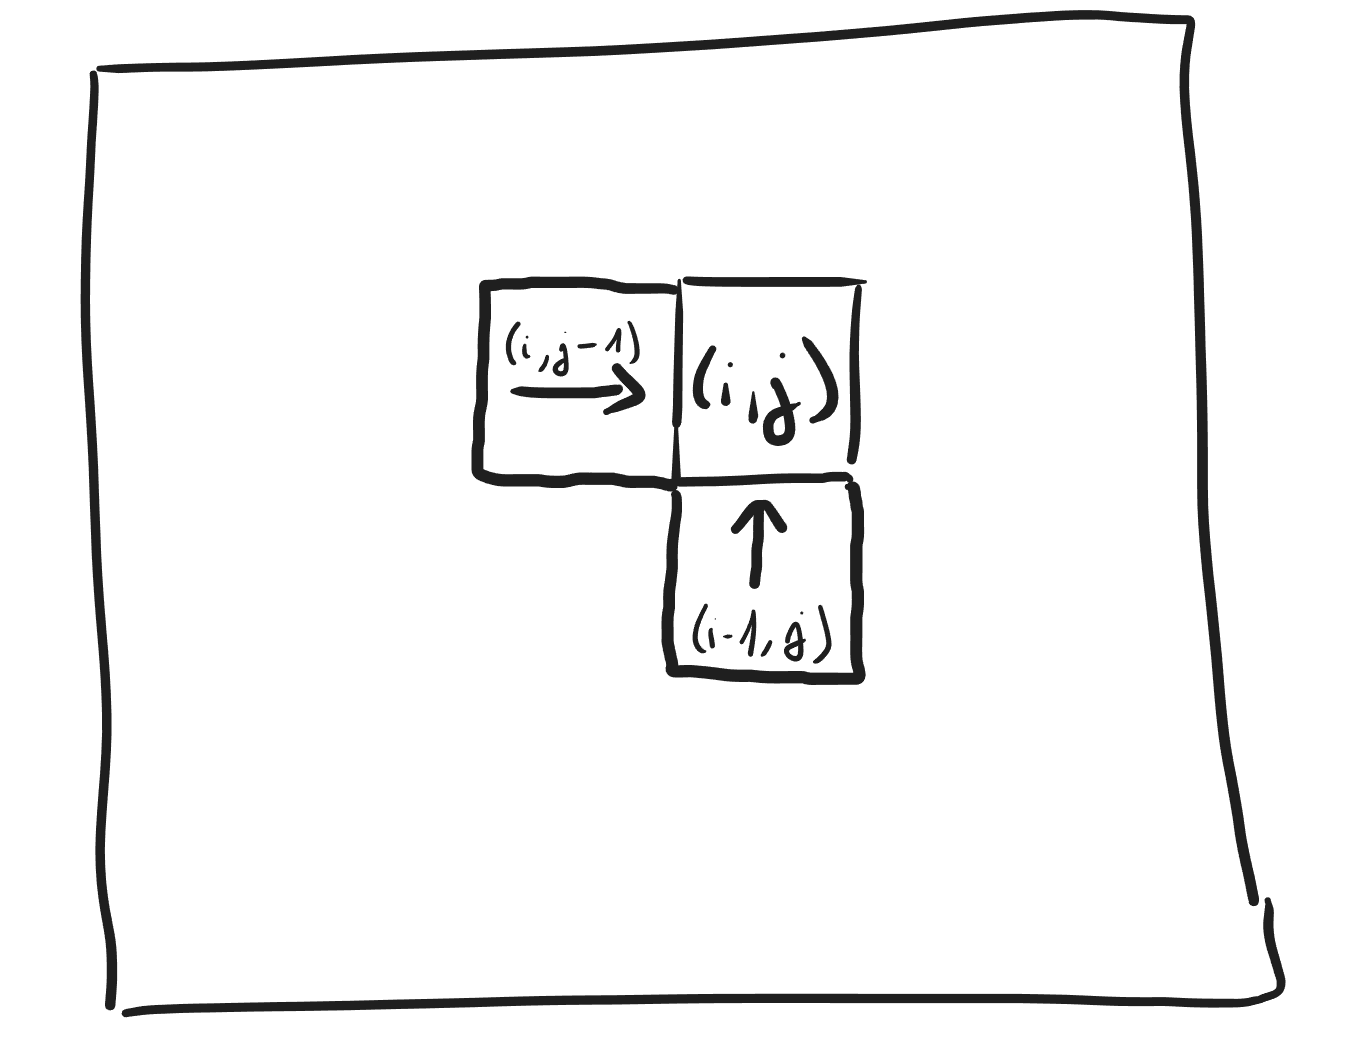
\includegraphics[width=\linewidth]{10/05/chess_recursive.png}
\end{center}

\begin{itemize}
    \item This does not yet take into account un-steppable cells. If $T[i,j]$ is unsteppable, we would like to zero out its value.
    \item Let's modify the previously introduced 2D board $B[i,j]$, and say that the value of $B[i,j]$ will be $1$ if that square is steppable and $0$ if not.
    \item Now we can simply multiply the result with $B[i,j]$, which will make the cell value zero if it's not steppable.
    \item $T[i,j] = B[i, j] \cdot{} (T[i, j-1] + T[i-1, j])$.
    \item What's left for us to do is:
    \begin{itemize}
        \item The above recursive formula relies on previous square values. This needs to start somewhere, so we need to give the base cases for the formula.
        \item We must give the order in which $T$ is filled out, so every time a cell is filled, we already have the needed previous values computed.
        \item We must say where the solution is in $T$. While in this exercise, the solution will be in $T[n,n]$, in other exercises it could be a maximum of all values in $T$, or other possibilities. See \nameref{exam_2022_05_30_exercise_7} for an example like this.
        \item Say what is the runtime of the resulting algorithm. Most exercises will ask us to give a specific $O(\dots{})$ to fulfill, so we need to show, that our algorithm fulfills this criteria.
    \end{itemize}
\end{itemize}

I like to summarize all of this into 6 steps, and this is what I would write down in the exam:

\begin{itemize}
    \item \textbf{Step 1}: Define the $T$ DP table. What does $T[i,j]$ mean?
    \begin{itemize}
        \item $T$ is a 2 dimensional table, of size $(n \times n)$.
        \item $T[i, j]$ contains the number of ways the square in the $i$th row and $j$th column is reachable from the bottom left square.
    \end{itemize}
    \item \textbf{Step 2}: Give the generic recursive formula. Explain why it is correct.
    \begin{itemize}
        \item $T[i,j] = B[i,j]\cdot{}(T[i, j-1] + T[i-1, j])$, for $i,j>1$.
        \item To step into the $(i,j)$ square, we could come from $(i,j-1)$ or $(i-1,j)$, so we add up the ways we could reach these cells.
        \item Then we multiply by $B[i,j]$, which is $0$ if $B[i,j]$ is not steppable, and $1$ if it is steppable. This means that non-steppable squares can be reached in $0$ ways, as intended.
        \item The formula only works if we are not in the first row or column, since in these cases, there is no left hand side or lower square. This is handled by the base cases instead.
    \end{itemize}
    \item \textbf{Step 3}: Give the base cases for the recursive formula (how to start filling out the array):
    \begin{itemize}
        \item $T[j,1] = 1$ and $T[1,j] = 1$ for all $1\leq{}j\leq{}n$.
        \item Explanation: $T[1,1] = 1$, since we start there, then this value is copied in the first row and column, since there is a single path to reach the squares here.
    \end{itemize}
    \item \textbf{Step 4}: The order in which $T$ must be filled.
    \begin{itemize}
        \item We can fill out $T$ by iterating the columns first, from $1$ to $n$, and inside each column iterate the rows from $1$ to $n$.
        \item This way the left and lower cells will already be computed for the current cell to use their value:
    \end{itemize}
\end{itemize}

\begin{center}
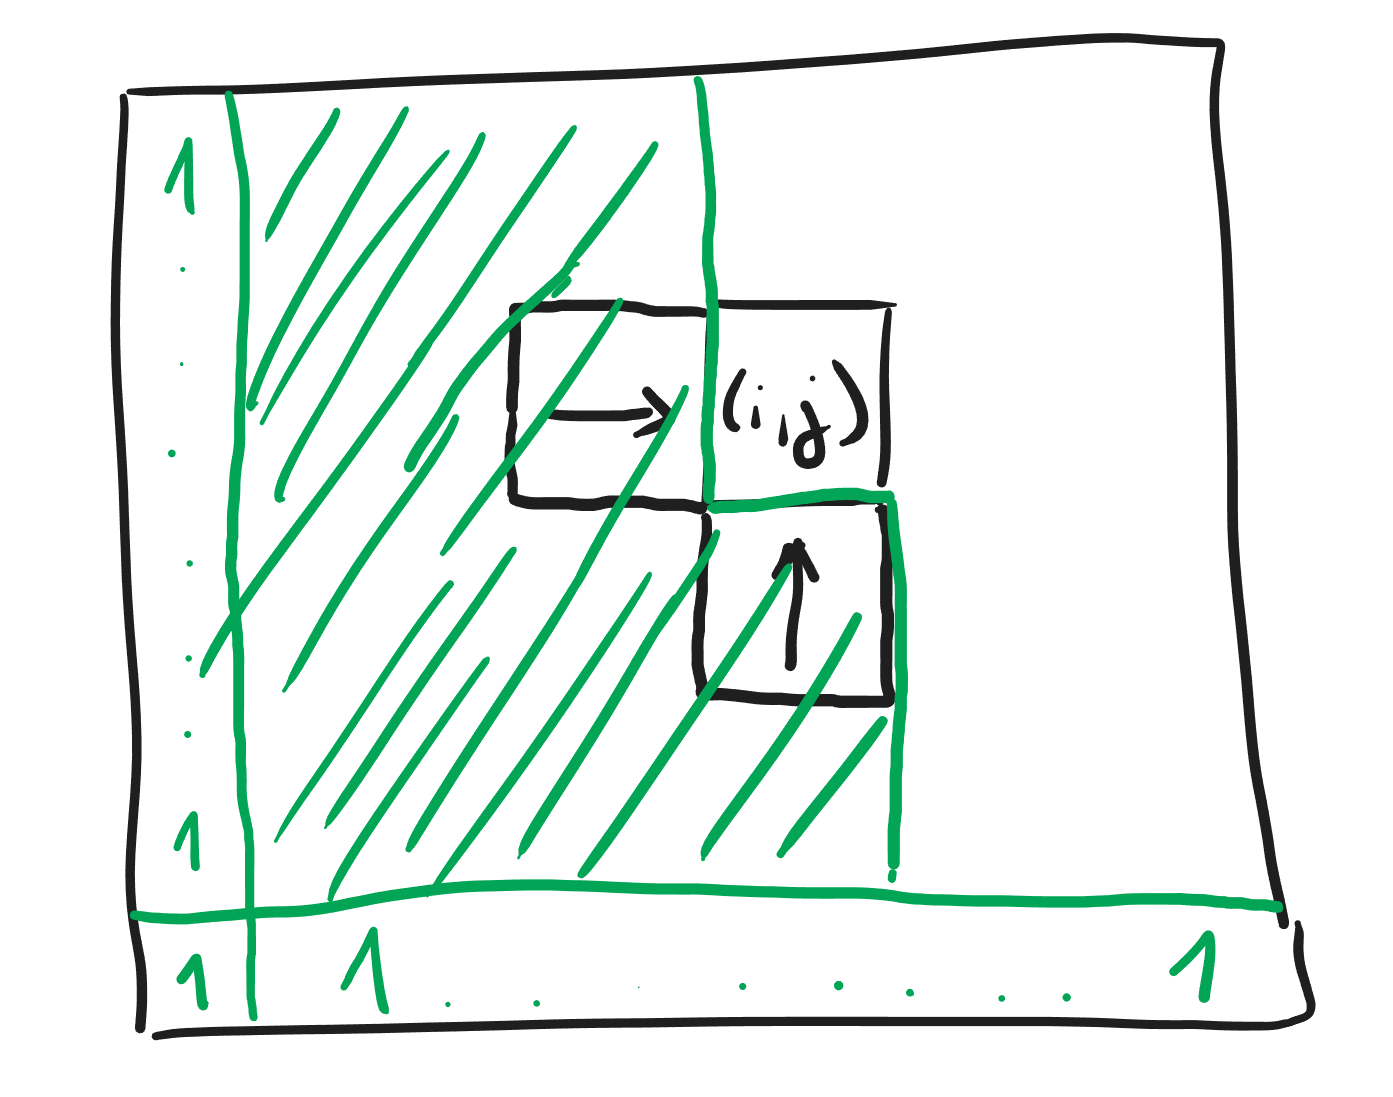
\includegraphics[width=\linewidth]{10/05/chess_order.png}
\end{center}

\begin{itemize}
    \item \textbf{Step 5}: Where is the solution in $T$?
    \begin{itemize}
        \item In $T[n,n]$, since that is how many ways we can reach the upper right square.
    \end{itemize}
    \item \textbf{Step 6}: What is the runtime of the algorithm?
    \begin{itemize}
        \item We fill out an $n^2$ sized table. In every step, we do an $O(1)$ calculation: we check on $2$ other values of the table, add them, multiply by $B[i,j]$. So in total, we do this in $O(n^2)$.
    \end{itemize}
    
\end{itemize}

